\section{Optimization of the PAU filter set}
\label{sec:opti}

In this section we want to explore how the photo-$z$ performance changes under variations of the PAU NB filter set. 

\subsection{NB filter set variations}
We study five variations of the original NB filter set whose response is shown in Fig.~\ref{pau_filt_sets}. All the variations conserve the number of filters. In the order that appear in Fig.~\ref{pau_filt_sets}, the proposed filter sets are:

\begin{table}
\centering
\caption{Global photo-$z$ performance results for each filter set shown in Fig.~\ref{pau_filt_sets}.  Photo-$z$ performance is characterized through the three metrics: bias (median), $\sigma_z$ ($\sigma_{68}$) and the $3\sigma$-outlier fraction. Photo-$z$ quality cuts resulting in a 50\% \ overall completeness are applied in all cases. We show results for the
Bright Sample (BS) and Faint Sample (FS).}
\begin{tabular}{lccc}
 & Bias & $\sigma_z$(\%) & Outliers(\%) \\
\hline
Default BS & -0.71$\cdot10^{-4}$ & 0.34 & 3.02
\\
Default FS & -1.33$\cdot10^{-3}$ & 4.73 & 7.36
\\
\hline
Blueshift BS &-2.11$\cdot10^{-4}$ & 0.38 &  3.23
\\
Blueshift FS & -3.11$\cdot10^{-3}$ & 5.19 & 7.05
\\
\hline
Redshift BS &-0.74$\cdot10^{-4}$  & 0.35 &   3.31
\\
Redshift FS &  -0.65$\cdot10^{-3}$  & 4.99 & 7.21
\\
\hline
Log BS &-0.69$\cdot10^{-4}$  & 0.35 &   2.80
\\
Log FS &  -1.46$\cdot10^{-3}$  & 4.73 & 7.43
\\
\hline
x1.5 width BS &-3.18$\cdot10^{-4}$  & 0.45 &   3.00
\\
x1.5 width FS &  -2.76$\cdot10^{-3}$  & 3.87 & 7.76
\\
\hline
x0.5 width BS &-0.00$\cdot10^{-4}$  & 0.32 &   5.22
\\
x0.5 width FS &  -0.99$\cdot10^{-3}$  & 6.91 & 5.52
\\
\hline
\end{tabular}
\label{tab:pz_results_filt_sets}
\end{table}

\begin{figure*}
\centering
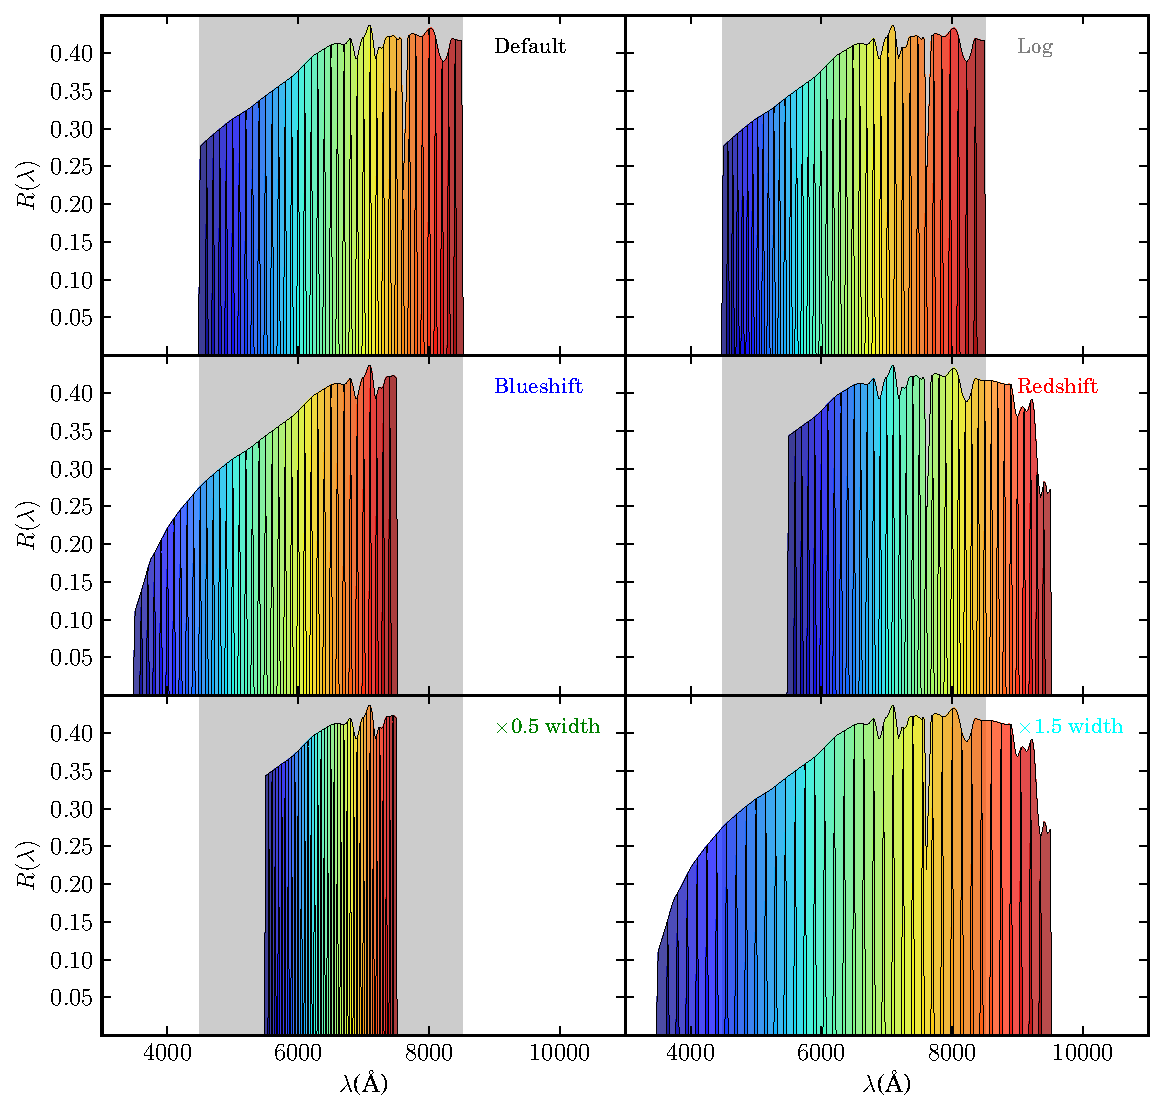
\includegraphics[height=130mm]{./plots/pau_filt_sets.pdf}
\caption{On the top-left, the original PAU NB filter set (same as in Fig.~\ref{pau_effective_bands}). The rest are the five variations to be compared in terms of photo-$z$ performance. Grayed areas show the covered wavelength range by the \texttt{Default} filter set. In descending order from left to right we have: the \texttt{Log} filter set with the same overall range as the \texttt{Default} but with band widths that increase logarithmically; the \texttt{Blueshift} filter set, which is the same as the \texttt{Default} but with the bands shifted 1000\AA \ towards bluer wavelengths; the \texttt{Redshift} filter set which is the same as \texttt{Default} but shifted towards redder wavelengths; the \texttt{$\times$0.5 width} filter set whose band widths are half those of the \texttt{Default} ones; and the \texttt{$\times$1.5 width} filter set whose bands are 1.5 times wider. The overall wavelength ranges of these last two set-ups are chosen to be centered with respect to the range of the \texttt{Default} set.}
\label{pau_filt_sets}
\end{figure*}

\begin{itemize}
\item \textbf{Default:} This is the default filter set already shown in Fig.~\ref{pau_effective_bands}. 
\item \textbf{Log:} In this filter set, band widths increase in wavelength logarithmically, so that they fulfill $\lambda_0 / \Delta \lambda=const.$, where $\Delta \lambda$ is the width of the rectangular part of the band (without taking into account the lateral wings) and $\lambda_0$ is the central wavelength of the band. We impose the overall wavelength range covered by the set of bands to be the same as for the \texttt{Default} filter set. Given that the total number of bands is kept at 40, we obtain that the bluest filter has a width of 97\AA, while the reddest is 159\AA \ wide. The reason for this filter set is that, when spectra are redshifted, their spectral features are moved to redder wavelengths, but also their widths are stretched as $\Delta \lambda ' = (1+z) \Delta \lambda$. If the photo-$z$ determination depends strongly on the tracking of any spectral feature, such as the 4000\AA \ break in elliptical galaxies, a filter set like \texttt{Log} will continue to enclose the same fraction of the spectral feature in a single filter independently of how redshifted is the spectrum.
\item \textbf{Blueshift:} This is the same as the \texttt{Default} filter set, however bands have been shifted 1000\AA \ towards bluer wavelengths. We expect to get better photo-$z$ performance at low redshift and for late-type galaxies. The down side of this filter set is that the overall response turns out to be very inefficient in the ultraviolet zone (middle-left of Fig.~\ref{pau_filt_sets}), like it was for the \textit{u} band.
\item \textbf{Redshift:} This is the same variation as before but shifting bands 1000\AA \ towards redder wavelengths. We expect to get better photo-$z$ performance at high redshift and for early-type galaxies. This filter set does not suffer from the problem of the ultraviolet, so its band responses are much more uniform over the covered range (middle-right of Fig.~\ref{pau_filt_sets}). On the other hand, the sky brightness on this region is higher.
\item \textbf{$\times$0.5 width:} This is a filter set whose band widths are half of the \texttt{Default} ones. Lateral wings are also reduced to half of their size, from 25\AA \ to 12.5\AA, in order to avoid an excessive overlap between adjacent bands. We expect to improve the photo-$z$ precision, at least for galaxies with good Signal-to-Noise ratio on their photometry. The down side of this filter set is that, since the number of bands is kept, the overall wavelength range covered is also reduced by a half. We choose it to be centered with respect to the \texttt{Default}, so that it covers from 5500\AA \ to 7500\AA, roughly spanning only from the bluest filter of the \texttt{Redshift} set to the reddest of the \texttt{Blueshift} set. This can lead to a degradation of the photo-$z$s at very low and high redshift, although the broad bands may attenuate this effect.
\item \textbf{$\times$1.5 width:} This is a filter set whose band widths are 1.5 times wider than the \texttt{Default} ones. Because of this, we expect a significant degradation of the photo-$z$ precision for galaxies with good Signal-to-Noise ratio on their photometry. However, the increase in $S/N$ may help. Moreover, the covered wavelength range also increases by 50\%. We choose the new range to be centered with respect to the \texttt{Default} set, so that it covers from 3500\AA \ to 9500\AA, roughly from the bluest edge of the \texttt{Blueshift} set to the reddest edge of the \texttt{Redshift} set, so we expect to see a more uniform photo-$z$ performance over the whole redshift range.
\end{itemize}

We generate magnitudes for each filter set band as described in Section~\ref{sec:mock} using the same exposure times per NB filter tray and BB as in the \texttt{Default} filter set. We do not try to optimize the exposure times for each filter set. The aim of this study is to see how, in spite of this, the photo-$z$ performance changes. Once the new photometric mock catalogs are created, they are also split into a Bright Sample ($i_{AB}<22.5$) and Faint Sample ($22.5<i_{AB}<23.7$). We run BPZ on each catalog using the same settings as for the \texttt{Default} filter set. There is no need to calibrate a different prior for each filter set, since the prior was initially calibrated on the broad band $i$, which is shared by all these filter sets. Photo-$z$ quality cuts resulting in an overall completeness of $\sim$50\% are applied in all cases.
\begin{figure*}
\centering
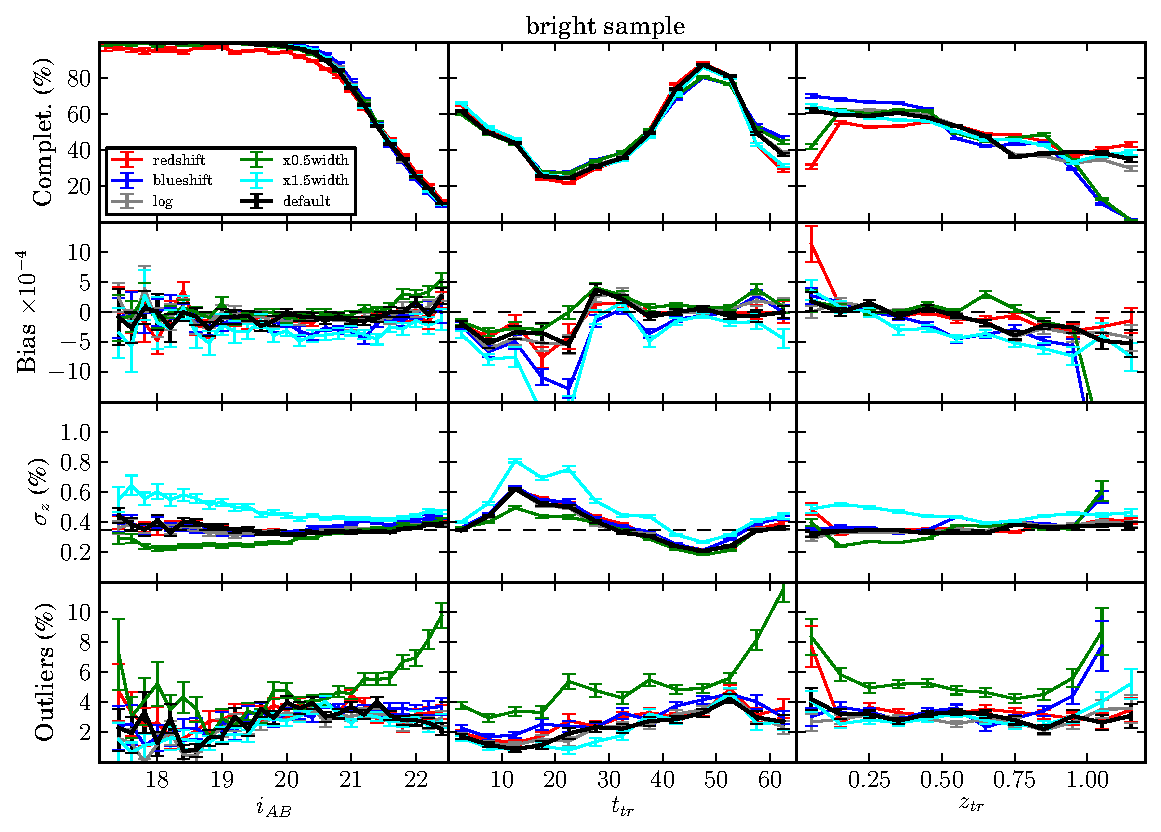
\includegraphics[type=pdf,ext=.pdf,read=.pdf, width=130mm]{./plots/mock.r260.n1e6.s10.121027_bright_filt_sets_compar} \\
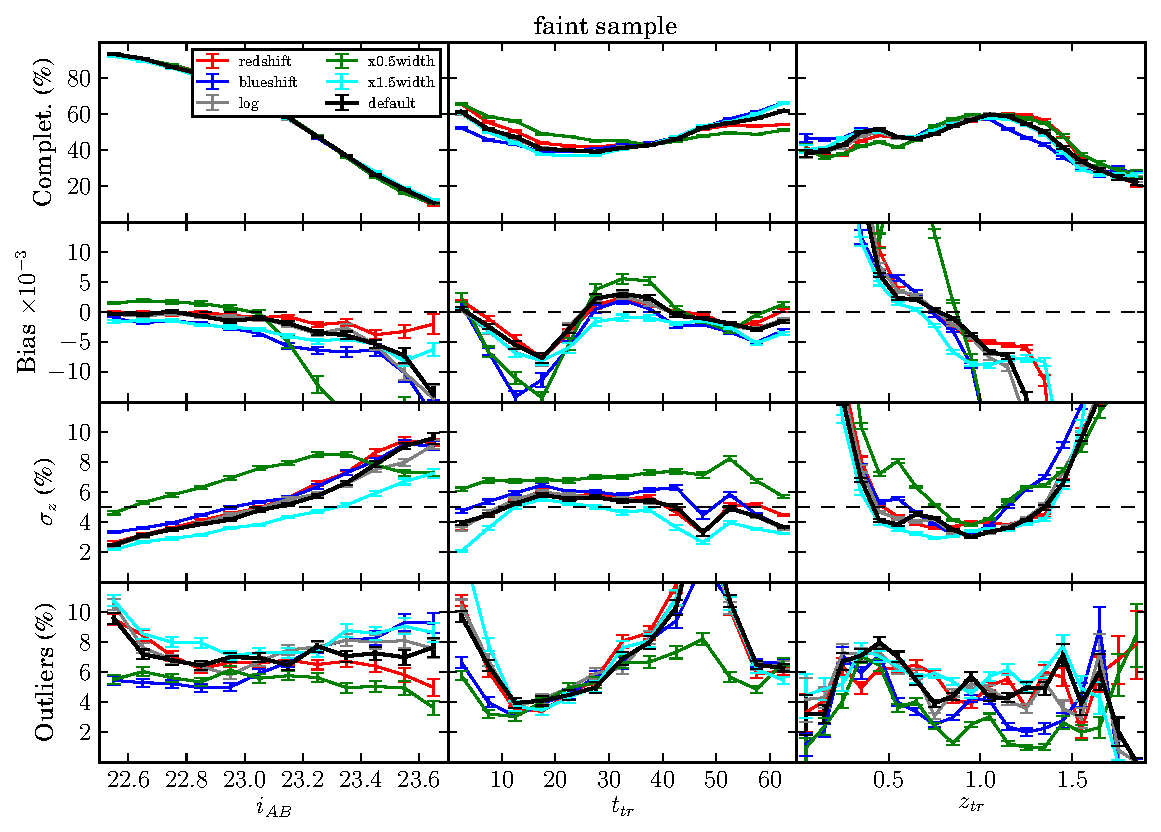
\includegraphics[type=pdf,ext=.pdf,read=.pdf, width=130mm]{./plots/mock.r260.n1e6.s10.121027_faint_filt_sets_compar}
\caption{Photo-$z$ performance metrics using the different filter sets shown in Fig.~\ref{pau_filt_sets}. Rows: Completeness after applying a photo-$z$ quality cut leading to a 50\% global completeness; bias (median); $\sigma_z$ ($\sigma_{68}$) and 3$\sigma$-outlier fraction, as a function of $i_{AB}$, $t_{tr}$ and $z_{tr}$ (columns), in the BS (top) and the FS (bottom).}
\label{pz_results_filt_sets}
\end{figure*}

\subsection{Global photo-$z$ performance}
Global photo-$z$ performance results for each filter set are shown on Table~\ref{tab:pz_results_filt_sets}, using the same metrics as in Section~\ref{sec:photoz}: bias (median), $\sigma_z$ ($\sigma_{68}$) and the $3\sigma$-outlier fraction. We find that the \texttt{$\times$0.5 width} set gives the best bias (it completely vanishes), and $\sigma_z$ ($\sim$6\% better than \texttt{Default}) in the BS, while in the FS it is the \texttt{Redshift} set which gives the best bias ($\sim$54\% better) and the \texttt{$\times$1.5 width} set which gives the best $\sigma_z$ ($\sim$18\% better). On the other hand, the \texttt{$\times$1.5 width} set gives the worst bias (a factor 4.6 worse) and $\sigma_z$ ($\sim$32\% worse) in the BS, while in the FS it is the \texttt{Blueshift} set which gives the worst bias (a factor 2.4 worse) and the \texttt{$\times$0.5 width} which gives the worst $\sigma_z$ ($\sim$46\% worse). Regarding the outlier fraction, its direct comparison is trickier since it depends on the value of $\sigma_z$. Even so, we see that in the BS the \texttt{Log} set gives the best value, while in the FS the \texttt{$\times$0.5 width} set gives the worst. 

The general conclusions are that the \texttt{Log} set gives almost the same photo-$z$ performance as the \texttt{Default} set, with a slight increase of $3\%$ in $\sigma_z$ in the BS. Therefore, we see that the logarithmic broadening of the band widths does not suppose any global improvement. On the other hand, and as we expected, if the Signal-to-Noise ratio in the photometry is good enough, the narrower the bands, the better the photo-$z$ performance results. On the other hand, wider bands are the ones that give better photo-$z$ precision in the FS, because there are more bands that pass the cut $\sigma_m<0.5$ introduced in Section~\ref{sec:mock}. 

\subsection{Results as a function of $i_{AB}$, $t_{tr}$ and $z_{tr}$}
In Fig.~\ref{pz_results_filt_sets} we show plots similar to those in Figs.~\ref{bs_pz_results} and \ref{fs_pz_results} with the photo-$z$ performance metrics as a function of $i_{AB}$, $t_{tr}$ and $z_{tr}$ for the BS (top) and the FS (bottom) when using the different filter sets of Fig.~\ref{pau_filt_sets}. Black curves correspond to the photo-$z$ results of the \texttt{Default} filter set when the 50\% completeness photo-$z$ quality cut is applied, and we will treat them as the reference results. The rest of curves in different colors correspond to the variations of the \texttt{Default} filter set. As a general trend, we see that these curves do not deviate much from the reference. Even so, we will discuss each case separately. 

In the BS, we see that redshifting the bands (red curves) slightly degrades the completeness at low magnitudes up to $i_{AB}<21.5$. As was expected, all the metrics also degrade at low $z_{tr}$. In contrast, blueshifting the bands (blue curves) shows the opposite behavior, a degradation of all the metrics at high $z_{tr}$. This is due to the lack of coverage at blue and red wavelengths respectively of each filter set, as we have already mentioned before. Something similar happens for the \texttt{$\times$0.5 width} set, where band widths, and consequently the covered wavelength range, is reduced by a half (green curve). The resulting photo-$z$ performance is worse at both low and high $z_{tr}$. However, the photo-$z$ precision $\sigma_z$ is slightly better at intermediate redshifts ($0.15<z_{tr}<0.5$), for spiral galaxies ($10<t_{tr}<30$) and at bright magnitudes ($i_{AB}<20.5$). Increasing the band width by a factor 1.5 (cyan curve) does not result in an improvement in any case. Bias and $\sigma_z$ degrade all over the range of the three variables, $i_{AB}$, $t_{tr}$ and $z_{tr}$. This is in full agreement with the results shown in Table~\ref{tab:pz_results_filt_sets}, where this filter set was seen as giving the worst photo-$z$ performance. Also in agreement with Table~\ref{tab:pz_results_filt_sets}, we see that the \texttt{Log} filter set practically does not introduce any change from the \texttt{Default} filter set. 

In the FS we do not observe big differences between the completeness curves, but for example the \texttt{Blueshift} filter set shows slightly lower completeness for elliptical galaxies than for irregulars, unlike the \texttt{Redshift} and \texttt{$\times$0.5 width} filter sets, which show the opposite behavior. In the $z_{tr}$ range we also recognize similar behaviors as in the BS, as for example the fact that the \texttt{Blueshift} filter set shows better completeness at low $z_{tr}$ and worse at high, as well as the opposite behavior of the \texttt{Redshift} and \texttt{$\times$0.5 width} filter sets. The \texttt{Blueshift} filter set seems to cause a significant degradation in the bias for faint, spiral and high redshift galaxies, and also delivers a considerably worse $\sigma_z$ than the \texttt{Default} over all the ranges. In return, the \texttt{Redshift} filter set shows better bias at high magnitudes and redshifts. On the other hand, we observe that the \texttt{$\times$0.5 width} filter set shows much more pronounced trends on the bias, in particular at $i_{AB}>23.1$, spiral galaxies and over all the $z_{tr}$ range, where values are substantially worse than for the \texttt{Default} filter set. As in Table~\ref{tab:pz_results_filt_sets}, we observe that the worst $\sigma_z$ is found for the \texttt{$\times$0.5 width} filter set, while the best is for the \texttt{$\times$1.5 width} filter set over all the ranges. This is exactly the opposite to the behavior seen for the BS. 
In general, narrower bands are useful in the BS, but not in the FS.  
